% mnras_template.tex 
%
% LaTeX template for creating an MNRAS paper
%
% v3.0 released 14 May 2015
% (version numbers match those of mnras.cls)
%
% Copyright (C) Royal Astronomical Society 2015
% Authors:
% Keith T. Smith (Royal Astronomical Society)

% Change log
%
% v3.0 May 2015
%    Renamed to match the new package name
%    Version number matches mnras.cls
%    A few minor tweaks to wording
% v1.0 September 2013
%    Beta testing only - never publicly released
%    First version: a simple (ish) template for creating an MNRAS paper

%%%%%%%%%%%%%%%%%%%%%%%%%%%%%%%%%%%%%%%%%%%%%%%%%%
% Basic setup. Most papers should leave these options alone.
\documentclass[fleqn,usenatbib]{mnras}

% MNRAS is set in Times font. If you don't have this installed (most LaTeX
% installations will be fine) or prefer the old Computer Modern fonts, comment
% out the following line
\usepackage{newtxtext,newtxmath}
% Depending on your LaTeX fonts installation, you might get better results with one of these:
%\usepackage{mathptmx}
%\usepackage{txfonts}

% Use vector fonts, so it zooms properly in on-screen viewing software
% Don't change these lines unless you know what you are doing
\usepackage[T1]{fontenc}

% Allow "Thomas van Noord" and "Simon de Laguarde" and alike to be sorted by "N" and "L" etc. in the bibliography.
% Write the name in the bibliography as "\VAN{Noord}{Van}{van} Noord, Thomas"
\DeclareRobustCommand{\VAN}[3]{#2}
\let\VANthebibliography\thebibliography
\def\thebibliography{\DeclareRobustCommand{\VAN}[3]{##3}\VANthebibliography}


%%%%% AUTHORS - PLACE YOUR OWN PACKAGES HERE %%%%%

% Only include extra packages if you really need them. Common packages are:
\usepackage{graphicx}	% Including figure files
\usepackage{amsmath}	% Advanced maths commands
\usepackage{amssymb}	% Extra maths symbols

%%%%%%%%%%%%%%%%%%%%%%%%%%%%%%%%%%%%%%%%%%%%%%%%%%

%%%%% AUTHORS - PLACE YOUR OWN COMMANDS HERE %%%%%

% Please keep new commands to a minimum, and use \newcommand not \def to avoid
% overwriting existing commands. Example:
%\newcommand{\pcm}{\,cm$^{-2}$}	% per cm-squared

%%%%%%%%%%%%%%%%%%%%%%%%%%%%%%%%%%%%%%%%%%%%%%%%%%

%%%%%%%%%%%%%%%%%%% TITLE PAGE %%%%%%%%%%%%%%%%%%%

% Title of the paper, and the short title which is used in the headers.
% Keep the title short and informative.
\title[Kilonova modeling with SNEC]{Radiation hydrodynamics modeling of kilonovae with SNEC}

% The list of authors, and the short list which is used in the headers.
% If you need two or more lines of authors, add an extra line using \newauthor
\author[Z.~Wu]{
Zhenyu Wu,$^{1}$\thanks{E-mail: 171840687\@smail.nju.edu.cn}
Full author list TBD
\\
% List of institutions
$^{1}$ Nanjing University\\
}

% These dates will be filled out by the publisher
\date{Accepted XXX. Received YYY; in original form ZZZ}

% Enter the current year, for the copyright statements etc.
\pubyear{2021}

% Don't change these lines
\begin{document}
\label{firstpage}
\pagerange{\pageref{firstpage}--\pageref{lastpage}}
\maketitle

% Abstract of the paper
\begin{abstract}
\textcolor{red}{Draft version, not for distribution}
\end{abstract}

% Select between one and six entries from the list of approved keywords.
% Don't make up new ones.
\begin{keywords}
keyword1 -- keyword2 -- keyword3
\end{keywords}

%%%%%%%%%%%%%%%%%%%%%%%%%%%%%%%%%%%%%%%%%%%%%%%%%%%%%%%%%%%%%%%%%%%%%%%%%%%%%

\begin{enumerate}
    \item Use bibtex keys from INSPIRE. I have a script to generate the bibtex automatically from those
    \item The section titles are just suggestions and will be finalized later
    \item Let's start with assembling the relevant plots and some text for the methods section
\end{enumerate}

% ===========================================================================
\section{Introduction}
% ===========================================================================

% ===========================================================================
\section{Methods}
% ===========================================================================
\begin{itemize}
    \item Brief overview of SNEC
    \item Opacities
    \item Heating rates\\
    At the times relevant for kilonovae, the ejecta has already lost all of its initial thermal energy at expansion, and the dominant source of heating is constituted by the decays of heavy elements produced in the r-process. This heating can be described by a specific heating rate which can be derived by evolving the system of the numerous characteristic nuclides in time while accounting for their mutual interactions.\\
    Here, time-dependent heating rates obtained using the nuclear reaction network SkyNet with a FRDM nuclear mass model are employed. A single SkyNet run is determined by the set of thermodynamic variables initial electron fraction $Y_e$, initial specific entropy $s$ and expansion timescale $\tau$. The rates are thus computed on a comprehensive grid with $0.02\leq Y_e\leq0.48$ linearly spaced, $1.82$ $\mathrm{k_B/baryon}$ $\leq s\leq100$ $\mathrm{k_B/baryon}$ and $1.36$ ms $\leq\tau\leq100$ ms log-spaced, the results on a representative subgrid being reported in Figure \ref{heatrates}.\\
    \begin{figure}
    \centering
    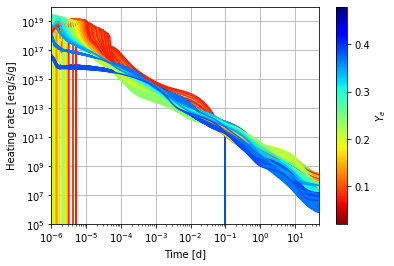
\includegraphics[scale=0.65]{heatrates.png}
    \caption{Heating rate trajectories as obtained by SkyNet on a subgrid of thermodynamic variables $0.05\leq Y_e\leq0.4$, $3$ $\mathrm{k_B/baryon}$ $\leq s\leq50$ $\mathrm{k_B/baryon}$ and $1$ ms $\leq\tau\leq30$ ms for visual clarity. Trajectories are color-coded to indicate different initial electron fractions. Vertical lines correspond to SkyNet noise which is averaged out in the fit procedure.}
    \label{heatrates}
    \end{figure}
    In order to derive the heating rate for arbitrary initial conditions, the above trajectories are reduced to a parametrized functional form by means of a fit procedure intended to cover the time interval from $0.1$ s to $50$ days post-merger, and, in particular, a distinction between time regimes is introduced. For early times $t\lesssim0.1$ days, the analytic fitting formula, derived from detailed nucleosynthesis calculations (\cite{Korobkin:2012uy}), is employed:
    \begin{equation}
    \label{eqKorfit}
    \dot{\epsilon}_{\mathrm{r}}(t)=\epsilon_0\epsilon_{\mathrm{th}}\left(\frac{1}{2}-\frac{1}{\pi}\arctan{\left[\frac{t-t_0}{\sigma}\right]}\right)^{\alpha},
    \end{equation}
    where $\epsilon_0$, $\alpha$, $t_0$ and $\sigma$ are considered fit parameters, while $\epsilon_{\mathrm{th}}<1$ is the thermalization efficiency. At late times $t\gtrsim0.1$ days instead, we expect a power-law fit to be a sufficiently good approximation of the heating rates, and thus the fitting formula becomes:
    \begin{equation}
    \label{eqpowfit}
    \dot{\epsilon}_{\mathrm{r}}(t)=\epsilon_0'\epsilon_{\mathrm{th}}t^{-\alpha'},
    \end{equation}
    with $\epsilon_0'$ and $\alpha'$ additional fit parameters.\\
    The heating rate fits, as obtained by using equations \ref{eqKorfit} and \ref{eqpowfit}, are then joint together with a log-scaled smoothing procedure applied on the time interval $1\times10^3$ s $\leq t\leq4\times10^4$ s, centered on $t\sim0.1$ days in log-scale.\\
    Figure \ref{heatratesfit} shows the fitted version of the heating rate trajectories presented in Figure \ref{heatrates}.
    \begin{figure}
    \centering
    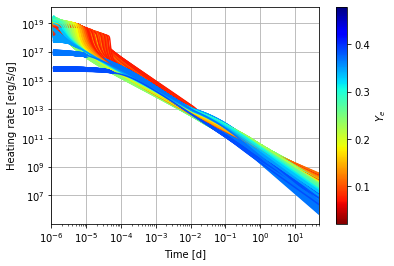
\includegraphics[scale=0.65]{heatratesfit.png}
    \caption{Heating rate fitted trajectories as obtained by performing the fit procedure on a subgrid of thermodynamic variables $0.05\leq Y_e\leq0.4$, $3$ $\mathrm{k_B/baryon}$ $\leq s\leq50$ $\mathrm{k_B/baryon}$ and $1$ ms $\leq\tau\leq30$ ms for visual clarity. Trajectories are color-coded to indicate different initial electron fractions.}
    \label{heatratesfit}
    \end{figure}
    %also possible plot with a bunch of characteristic trajectories superimposed to their fit along with fit error
    
    
    \item Initial and boundary conditions
\end{itemize}

% ===========================================================================
\section{Code validation}
% ===========================================================================
\subsection{Hydrodynamics}
\subsection{Energy conservation}
\subsection{Comparison with analytic models}

% ===========================================================================
\section{Ab-initio simulations: from mergers to kilonovae}
% ===========================================================================
\subsection{General features}
\subsection{Impact of uncertainties in the heating rates}

% ===========================================================================
\section{A first application to AT2017gfo}
% ===========================================================================
\subsection{Best fitting analytical models}
\subsection{Comparison between NR informed models and observations}
\subsection{Impact of shock cooling}

% ===========================================================================
\section{Conclusions}
% ===========================================================================

\bibliographystyle{mnras}
\bibliography{references}


% Don't change these lines
\bsp	% typesetting comment
\label{lastpage}
\end{document}

% End of mnras_template.tex
